\documentclass[11pt,aspectratio=169]{beamer}

% Core packages
\usepackage{amsmath,amssymb}
\usepackage{tikz-cd}
\usepackage{animate}
\usepackage{multicol}
\usepackage{lmodern}
\usepackage[T1]{fontenc}

% Color palette
\definecolor{Ink}{HTML}{14243A}
\definecolor{Midnight}{HTML}{10253F}
\definecolor{Teal}{HTML}{16B8A6}
\definecolor{Coral}{HTML}{F47763}
\definecolor{Gold}{HTML}{F2B84B}
\definecolor{Mist}{HTML}{F3F7FA}
\definecolor{Muted}{HTML}{64748B}

% Clean, spacious slide styling
\setbeamercolor{normal text}{fg=Ink,bg=white}
\setbeamercolor{structure}{fg=Teal}
\setbeamercolor{frametitle}{fg=Ink,bg=white}
\setbeamercolor{block title}{fg=white,bg=Midnight}
\setbeamercolor{block body}{fg=Ink,bg=Mist}
\setbeamercolor{alerted text}{fg=Coral}
\setbeamercolor{recall}{fg=Ink,bg=Mist}
\setbeamerfont{frametitle}{series=\bfseries,size=\Large}
\setbeamertemplate{navigation symbols}{}
\setbeamertemplate{itemize item}{\color{Teal}\raisebox{0.15ex}{\small\textbullet}}
\setbeamertemplate{itemize subitem}{\color{Coral}\raisebox{0.15ex}{\tiny\textbullet}}
\setbeamertemplate{frametitle}{%
  \vspace{0.68cm}
 % 1. Autor-Zeile mit unsichtbarem Platzhalter (hält den vertikalen Abstand exakt ein)
  \noindent\makebox[\linewidth][s]{%
    {\color{Muted}\fontsize{7}{8}\selectfont\insertauthor}%
    \hfill\phantom{\sectionprogress}% Hält den Raum frei, rendert aber nichts
  }\par
  \vspace{0.18cm}%
  \insertframetitle\par
  \vspace{0.12cm}%
  {\color{Teal}\rule{0.12\paperwidth}{2.2pt}}%
  \hfill{\color{Coral}\rule{0.035\paperwidth}{2.2pt}}%
  \vspace{0.18cm}%
}
\setbeamertemplate{footline}{%
  \leavevmode%
  \hbox{%
    \begin{beamercolorbox}[wd=\paperwidth,ht=2.8ex,dp=1.2ex,leftskip=0.7cm,rightskip=0.7cm]{normal text}%
      {\color{Muted}\scriptsize%
        \ifx\insertsection\empty\relax\else
          \insertsection%
          \ifx\insertsubsection\empty\relax\else
            \ -- \insertsubsection%
          \fi
        \fi
      }%
      \hfill{\color{Muted}\scriptsize\insertframenumber}%
    \end{beamercolorbox}%
  }%
}
\setbeamersize{text margin left=0.8cm,text margin right=0.8cm}

\newcommand{\sectionprogress}{%
  \pgfmathtruncatemacro{\currentsectionframe}{\insertpagenumber-\insertsectionstartpage+1}%
  \pgfmathtruncatemacro{\totalsectionframes}{\insertsectionendpage-\insertsectionstartpage+1}%
  \pgfmathsetlengthmacro{\sectionprogresswidth}{1.15cm*\currentsectionframe/\totalsectionframes}%
  
\begin{tikzpicture}[baseline=-0.5ex]
    \fill[Mist] (0,0) rectangle (1.15cm,1.2pt);
    \fill[Teal] (0,0) rectangle (\sectionprogresswidth,1.2pt);
  \end{tikzpicture}%
  \hspace{0.25em}\currentsectionframe/\totalsectionframes
}
\newcommand{\recallbox}[2][Recall]{%
  \begin{beamercolorbox}[wd=\linewidth,sep=0.65em,rounded=true]{recall}%
    {\color{Coral}\scriptsize\bfseries #1}\hspace{0.65em}%
    {\small #2}%
  \end{beamercolorbox}%
}



% --- Globale Schalter für aktive Tools & Sichtbarkeit ---
\gdef\isactiveCalculus{0}
\gdef\isactivePDE{0}
\gdef\isactiveAbleitung{0}
\gdef\isactiveMarkov{0}
\gdef\isactiveMartingale{0}
\gdef\isactiveRueckwaerts{0}
\gdef\isactiveSobolev{0}
\gdef\ToolboxVisible{1} % 1 = sichtbar, 0 = versteckt

% Befehl zum Ausblenden auf der aktuellen Folie
\newcommand{\hidetoolbox}{\gdef\ToolboxVisible{0}}

% --- Toolbox Icons für den Einsatz im Text ---
% Beim Aufruf wird das Icon gezeichnet UND das Tool in der Toolbox vergrößert
\newcommand{\iconCalculus}{%
  \gdef\isactiveCalculus{1}%
  
\begin{tikzpicture}[baseline=-0.6ex]
    \fill[Teal] (0,0) circle (0.144cm);
  \end{tikzpicture}%
}
\newcommand{\iconPDE}{%
  \gdef\isactivePDE{1}%
  
\begin{tikzpicture}[baseline=-0.6ex]
    \fill[Coral] (-0.132cm,-0.132cm) rectangle (0.132cm,0.132cm);
  \end{tikzpicture}%
}
\newcommand{\iconAbleitung}{%
  \gdef\isactiveAbleitung{1}%
  
\begin{tikzpicture}[baseline=-0.6ex]
    \fill[Gold] (0,0.156cm) -- (-0.156cm,-0.12cm) -- (0.156cm,-0.12cm) -- cycle;
  \end{tikzpicture}%
}
\newcommand{\iconMarkov}{%
  \gdef\isactiveMarkov{1}%
  
\begin{tikzpicture}[baseline=-0.6ex]
    \fill[Ink] (0,0.156cm) -- (0.156cm,0) -- (0,-0.156cm) -- (-0.156cm,0) -- cycle;
  \end{tikzpicture}%
}
\newcommand{\iconMartingale}{%
  \gdef\isactiveMartingale{1}%
  
\begin{tikzpicture}[baseline=-0.6ex]
    \fill[Teal] (0,-0.156cm) -- (-0.156cm,0.12cm) -- (0.156cm,0.12cm) -- cycle;
  \end{tikzpicture}%
}
\newcommand{\iconRueckwaerts}{%
  \gdef\isactiveRueckwaerts{1}%
  
\begin{tikzpicture}[baseline=-0.6ex]
    \fill[Coral] (0,0.156cm) -- (0.132cm,0.078cm) -- (0.132cm,-0.078cm) -- (0,-0.156cm) -- (-0.132cm,-0.078cm) -- (-0.132cm,0.078cm) -- cycle;
  \end{tikzpicture}%
}
\newcommand{\iconSobolev}{%
  \gdef\isactiveSobolev{1}%
  
\begin{tikzpicture}[baseline=-0.6ex]
    \fill[Gold] (0,0.156cm) -- (0.144cm,0.048cm) -- (0.096cm,-0.12cm) -- (-0.096cm,-0.12cm) -- (-0.144cm,0.048cm) -- cycle;
  \end{tikzpicture}%
}

% --- Toolbox Logik ---
\newcommand{\toolbox}{%
  \ifnum\ToolboxVisible=1
    \begin{tikzpicture}[remember picture, overlay]
      % Fortschritt der aktuellen Section berechnen
      \pgfmathtruncatemacro{\currentsec}{\value{section}}
      \pgfmathtruncatemacro{\currframe}{\insertpagenumber-\insertsectionstartpage+1}
      \pgfmathtruncatemacro{\totframes}{\insertsectionendpage-\insertsectionstartpage+1}
      \pgfmathsetmacro{\secprog}{ifthenelse(\totframes>0, \currframe/\totframes, 1)}
      
      % Toolbox Hintergrund
      \node[
        anchor=north east,
        xshift=-0.4cm, yshift=-0.4cm,
        draw=Midnight, thick, fill=Mist, rounded corners=3.5pt,
        inner xsep=4pt, inner ysep=3pt,
        minimum width=8.4cm, minimum height=1.15cm
      ] (toolbox) at (current page.north east) {};
      
      % Titel der Toolbox
      \node[anchor=north, font=\sffamily\fontsize{5.5}{6}\bfseries, text=Midnight, yshift=9pt] at (toolbox.north) {TOOLBOX};
      
      \begin{scope}[shift={(toolbox.center)}, yshift=-0.20cm] 
        
        % 1. (Sec 2) - Teal, Kreis
        \begin{scope}[xshift=-3.30cm]
          \node[anchor=south, font=\sffamily\fontsize{4.2}{5.0}\selectfont, text=Midnight, align=center] at (0, 0.20cm) {Stochastic\\Calculus};
          \def\radius{0.144cm}
          \ifnum\isactiveCalculus=1
            \draw[black, very thick] (0,0) circle (\radius);
          \else
            \draw[Teal, thick] (0,0) circle (\radius);
          \fi
          \pgfmathsetmacro{\fillamt}{ifthenelse(\currentsec > 2, 1, ifthenelse(\currentsec == 2, \secprog, 0))}
          \begin{scope}
            \clip (-0.25,-0.25) rectangle (0.25, {-0.144 + 0.288*\fillamt});
            \fill[Teal] (0,0) circle (\radius);
          \end{scope}
        \end{scope}

        % 2. (Sec 3) - Coral, Quadrat
        \begin{scope}[xshift=-2.20cm]
          \node[anchor=south, font=\sffamily\fontsize{3.8}{4.5}\selectfont, text=Midnight, align=center] at (0, 0.20cm) {Partielle\\Differential-\\gleichungen};
          \def\size{0.132cm}
          \ifnum\isactivePDE=1
            \draw[black, very thick] (-\size,-\size) rectangle (\size,\size);
          \else
            \draw[Coral, thick] (-\size,-\size) rectangle (\size,\size);
          \fi
          \pgfmathsetmacro{\fillamt}{ifthenelse(\currentsec > 3, 1, ifthenelse(\currentsec == 3, \secprog, 0))}
          \begin{scope}
            \clip (-0.25,-0.25) rectangle (0.25, {-0.132 + 0.264*\fillamt});
            \fill[Coral] (-\size,-\size) rectangle (\size,\size);
          \end{scope}
        \end{scope}
        
        % 3. (Sec 4) - Gold, Dreieck nach oben
        \begin{scope}[xshift=-1.10cm]
          \node[anchor=south, font=\sffamily\fontsize{3.8}{4.5}\selectfont, text=Midnight, align=center] at (0, 0.20cm) {Markov\\Prozesse};
          \def\tripath{(0, 0.156cm) -- (-0.156cm, -0.12cm) -- (0.156cm, -0.12cm) -- cycle}
          \ifnum\isactiveAbleitung=1
            \draw[black, very thick] \tripath;
          \else
            \draw[Gold, thick] \tripath;
          \fi
          \pgfmathsetmacro{\fillamt}{ifthenelse(\currentsec > 4, 1, ifthenelse(\currentsec == 4, \secprog, 0))}
          \begin{scope}
            \clip (-0.25,-0.25) rectangle (0.25, {-0.12 + 0.276*\fillamt});
            \fill[Gold] \tripath;
          \end{scope}
        \end{scope}
        
        % 4. (Sec 5) - Ink, Raute
        \begin{scope}[xshift=0cm]
          \node[anchor=south, font=\sffamily\fontsize{4.2}{5.0}\selectfont, text=Midnight, align=center] at (0, 0.20cm) {Rückwärts\\Prozess};
          \def\diapath{(0, 0.156cm) -- (0.156cm, 0) -- (0, -0.156cm) -- (-0.156cm, 0) -- cycle}
          \ifnum\isactiveMarkov=1
            \draw[black, very thick] \diapath;
          \else
            \draw[Ink, thick] \diapath;
          \fi
          \pgfmathsetmacro{\fillamt}{ifthenelse(\currentsec > 5, 1, ifthenelse(\currentsec == 5, \secprog, 0))}
          \begin{scope}
            \clip (-0.25,-0.25) rectangle (0.25, {-0.156 + 0.312*\fillamt});
            \fill[Ink] \diapath;
          \end{scope}
        \end{scope}

        % 5. (Sec 6) - Teal, Dreieck nach unten
        \begin{scope}[xshift=1.10cm]
          \node[anchor=south, font=\sffamily\fontsize{4.2}{5.0}\selectfont, text=Midnight, align=center] at (0, 0.20cm) {Zusammenführung \\ SDEs u. PDEs};
          \def\invtripath{(0, -0.156cm) -- (-0.156cm, 0.12cm) -- (0.156cm, 0.12cm) -- cycle}
          \ifnum\isactiveMartingale=1
            \draw[black, very thick] \invtripath;
          \else
            \draw[Teal, thick] \invtripath;
          \fi
          \pgfmathsetmacro{\fillamt}{ifthenelse(\currentsec > 6, 1, ifthenelse(\currentsec == 6, \secprog, 0))}
          \begin{scope}
            \clip (-0.25,-0.25) rectangle (0.25, {-0.156 + 0.276*\fillamt});
            \fill[Teal] \invtripath;
          \end{scope}
        \end{scope}

        % 6. (Sec 7) - Coral, Hexagon
        \begin{scope}[xshift=2.20cm]
          \node[anchor=south, font=\sffamily\fontsize{4.2}{5.0}\selectfont, text=Midnight, align=center] at (0, 0.20cm) {Schwache\\Ableitungen\\u. Lösungen};
          \def\hexpath{(0, 0.156cm) -- (0.132cm, 0.078cm) -- (0.132cm, -0.078cm) -- (0, -0.156cm) -- (-0.132cm, -0.078cm) -- (-0.132cm, 0.078cm) -- cycle}
          \ifnum\isactiveRueckwaerts=1
            \draw[black, very thick] \hexpath;
          \else
            \draw[Coral, thick] \hexpath;
          \fi
          \pgfmathsetmacro{\fillamt}{ifthenelse(\currentsec > 7, 1, ifthenelse(\currentsec == 7, \secprog, 0))}
          \begin{scope}
            \clip (-0.25,-0.25) rectangle (0.25, {-0.156 + 0.312*\fillamt});
            \fill[Coral] \hexpath;
          \end{scope}
        \end{scope}
        
        % 7. (Sec 8) - Gold, Fünfeck
        \begin{scope}[xshift=3.30cm]
          \node[anchor=south, font=\sffamily\fontsize{4.2}{5.0}\selectfont, text=Midnight, align=center] at (0, 0.20cm) {Martingale\\Problem};
          \def\pentapath{(0, 0.156cm) -- (0.144cm, 0.048cm) -- (0.096cm, -0.12cm) -- (-0.096cm, -0.12cm) -- (-0.144cm, 0.048cm) -- cycle}
          \ifnum\isactiveSobolev=1
            \draw[black, very thick] \pentapath;
          \else
            \draw[Gold, thick] \pentapath;
          \fi
          \pgfmathsetmacro{\fillamt}{ifthenelse(\currentsec > 8, 1, ifthenelse(\currentsec == 8, \secprog, 0))}
          \begin{scope}
            \clip (-0.25,-0.25) rectangle (0.25, {-0.12 + 0.276*\fillamt});
            \fill[Gold] \pentapath;
          \end{scope}
        \end{scope}

      \end{scope}
    \end{tikzpicture}%
  \fi
  
  % Zwingender globaler Reset ALLER Schalter am Ende der Folie
  \gdef\isactiveCalculus{0}%
  \gdef\isactivePDE{0}%
  \gdef\isactiveAbleitung{0}%
  \gdef\isactiveMarkov{0}%
  \gdef\isactiveMartingale{0}%
  \gdef\isactiveRueckwaerts{0}%
  \gdef\isactiveSobolev{0}%
  \gdef\ToolboxVisible{1}% <-- Setzt die Toolbox für die NÄCHSTE Folie/Overlay automatisch wieder auf sichtbar
}
\addtobeamertemplate{footline}{}{\toolbox}



\title{Time Reversal of Diffusions}
\subtitle{Schwache Lösungen von Diffusionprozessen}
\author{Arne Huckemann}
\date{06.11.2026}

\begin{document}

{\setbeamertemplate{footline}{}
\begin{frame}[plain]
  \begin{tikzpicture}[remember picture,overlay]
    \fill[Midnight] (current page.south west) rectangle (current page.north east);
    \fill[Teal] (current page.north west) rectangle ([yshift=-0.16cm]current page.north east);
    \fill[Coral] ([xshift=0.78\paperwidth]current page.south west) rectangle (current page.south east);
    \fill[Gold] ([xshift=0.72\paperwidth]current page.south west) rectangle ([xshift=0.78\paperwidth,yshift=0.08cm]current page.south west);
    \fill[Teal,opacity=0.16] ([xshift=0.68\paperwidth,yshift=0.38\paperheight]current page.south west) circle (2.2cm);
    \fill[Coral,opacity=0.14] ([xshift=0.82\paperwidth,yshift=0.62\paperheight]current page.south west) circle (1.2cm);
  \end{tikzpicture}
  \vspace*{1.3cm}
  {\color{Teal}\large\textsc{Universität Mannheim}}\par
  \vspace{0.45cm}
  {\color{white}\huge\bfseries\inserttitle}\par
  \vspace{0.28cm}
  {\color{white!75}\large\insertsubtitle}\par
  \vfill
  {\color{white}\normalsize\insertauthor}\hspace{0.7em}
  {\color{white!55}\small\textbullet}\hspace{0.7em}
  {\color{white!75}\normalsize\insertdate}
  \vspace{0.8cm}
\end{frame}}



\section{Motivation}

\begin{frame}{Idee von Diffusion}\hidetoolbox
\begin{minipage}[c]{0.50\linewidth}{\tiny
 \begin{itemize}
      \item Wir wollen eine Verteilung $Y \sim \mu$ lernen
      \item Idee: Verrausche eine Verteilung, bis nur noch eine Normalverteilung übrig ist
      \item $f$ ist irgend eine Abbildung, die $Y$ über die Zeit $t$ verrauscht:
      \[
      f(Y,t) \to Z \sim \mathcal{N}(0,1), \quad \text{für } t \to \infty
      \]
      \item Finde die inverse $f^{-1}$ und generiere von $\mu$ samples, indem aus $Z \sim \mathcal{N}(0,1)$ hoffentlich gilt
      \[
      f^{-1} (Z,t) \to Y \sim \mu, \quad \text{für } t \to \infty. 
      \]
    \end{itemize}}
\end{minipage}\hfill
\begin{minipage}[c]{0.50\linewidth}
\begin{figure}[h]
    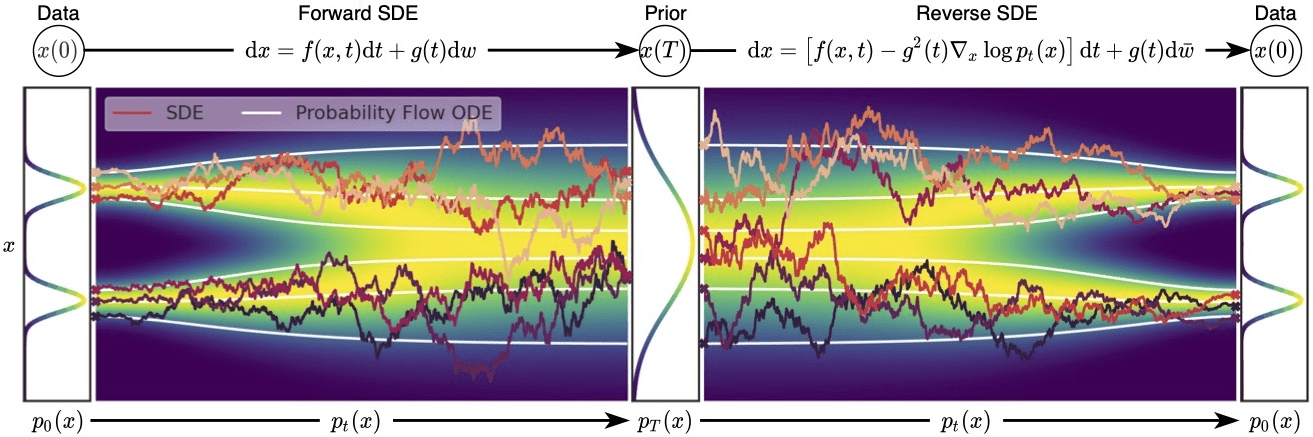
\includegraphics[width=0.9\textwidth]{Bilder/4.png} 
\end{figure}
\end{minipage}
\end{frame}



\begin{frame}{Präziesere Formulierung}\hidetoolbox

Für die Anfangsverteilung $X_0 \sim \mathbb{P}_0$ löst die forwärts Diffusion $(X_t)_{t \geq 0}$ die Differentialgleichung
\[
dX_t =b(X_t) dt + \sigma(X_t) dW_t, \quad X_t \sim p(\cdot,t)
\]
wobei $(W_t)_{t \geq 0}$ Brownsche Bewegung bzgl. $(\mathcal{F}_t)_{t \geq 0}$.\\
Der Rückwärtsprozess ist definiert als $\bar{X}_t := X_{T-t}$ und wir werden zeigen, dass dieser die folgende Differentialgleichung erfüllt.
\[
d\bar{X}_t = \underbrace{(-b(\bar{X_t}+ \sigma(\bar{X}_t)^2 \nabla \log(p(T-t,\bar{X}_t) )}_{=: \bar{b}(\bar{X}_t)} dt + \sigma(\bar{X}_t) d \tilde{W}_{t}, \quad X_t \sim \bar{p}(\cdot,t), 
\]
wobei $\tilde{W}_t$ Brownsche Bewegung bzgl. Rückwärtsfiltration $\bar{\mathcal{F}_t}$.
\end{frame}

\begin{frame}{Wir beantworten heute folgende Fragen}\hidetoolbox
\begin{itemize}
  \item Was ist eine Differentialgleichung?
  \item Wie sieht die marginale Verteilung $X_t \sim p(\cdot,t)$ aus und welche Probleme entstehen dort?
  \item Wie können wir dieses Problem lösen? Stichwort: Partielle Differentialgleichungen 
  \item Welche Differentialgleichung löst der Rückwärtsprozess und welche Eigenschaften erfüllt die Lösung.
\end{itemize}
\end{frame}

\begin{frame}{Interessant, aber nicht Thema heute}\hidetoolbox

\begin{minipage}[c]{0.52\linewidth}{\small
 \begin{itemize}
      \item Das Ziel: Beim Rückwärtsprozess die Score-function $\nabla \log(p(t,x))$ zu lernen. 
      \item Idee: Parametrisiere die Score-function durch $s_\theta (x,t)$ und minimiere
       \[
\mathbb{E}^{t \sim \mathcal{U}([0,T])} [ \mathbb{E}^{X_t \sim p(t,\cdot)} [ \| \nabla \log(p(t,x) - s_\theta(t,x) \|_2^2 ] ] 
\]
    \end{itemize}}
\end{minipage}\hfill
\begin{minipage}[c]{0.42\linewidth}
\begin{figure}[h]
    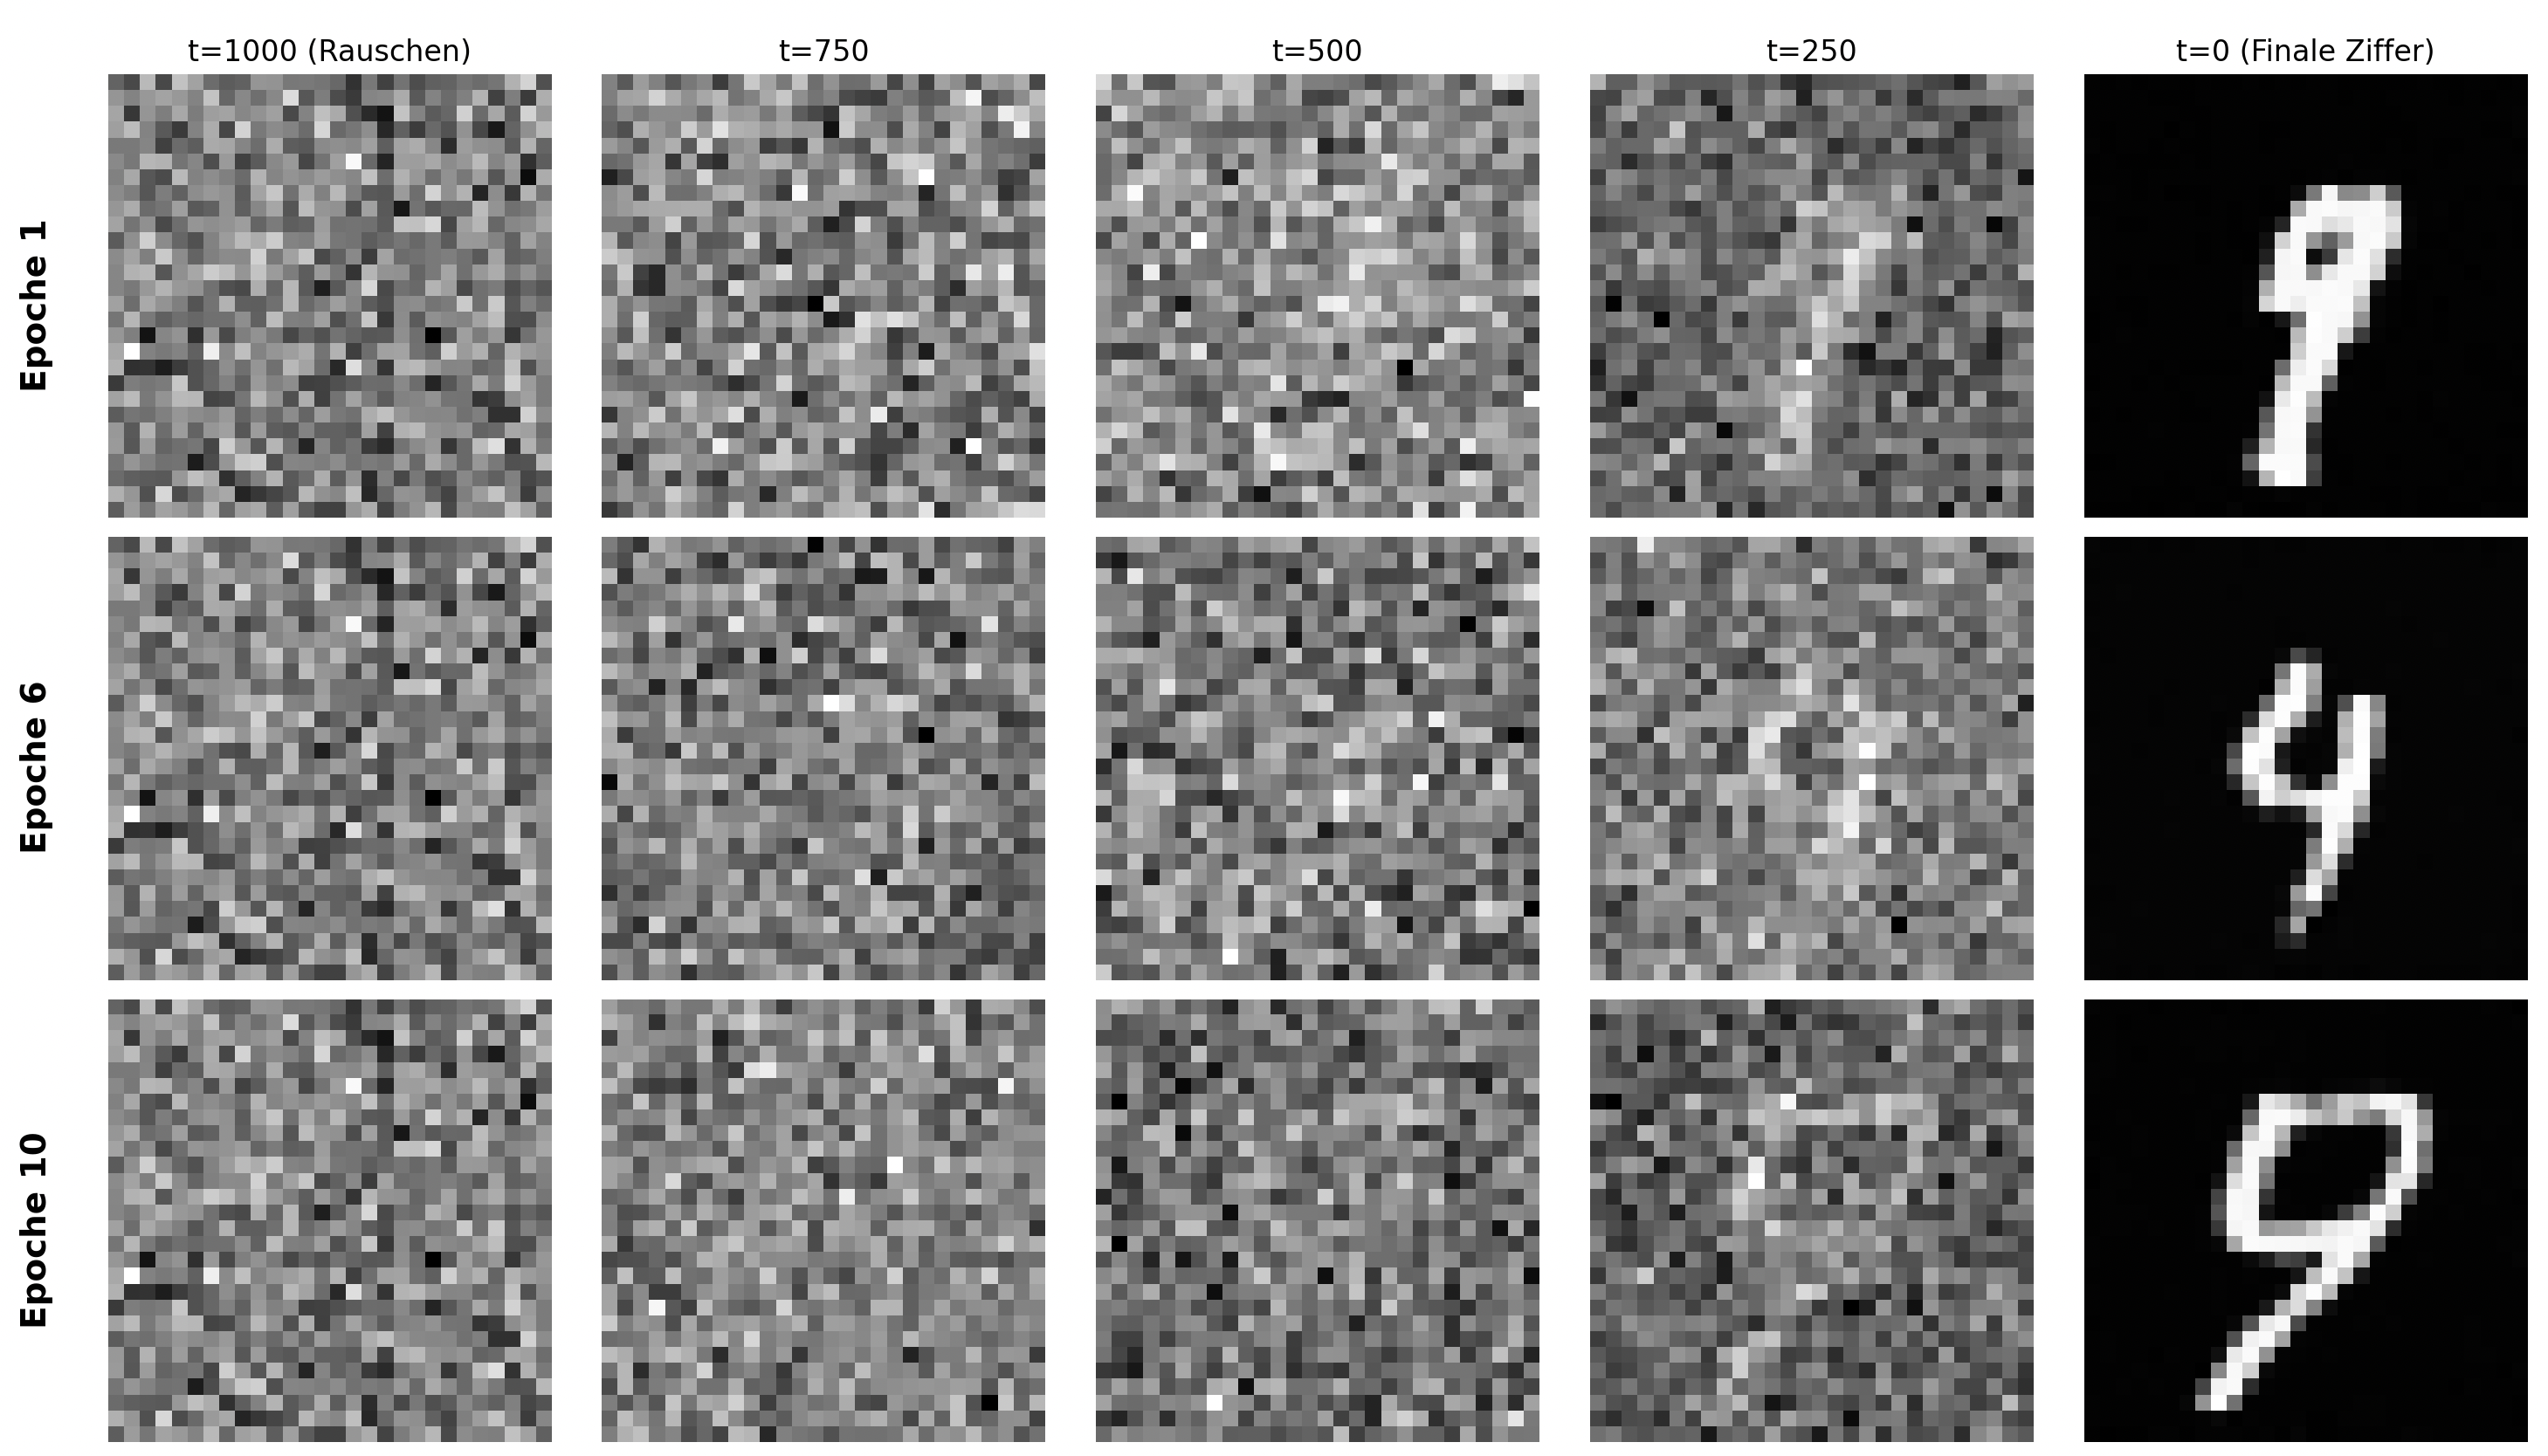
\includegraphics[width=1\textwidth]{Bilder/3.png} 
\end{figure}
\end{minipage}
\recallbox[Erinnerung:]{\small
$d\bar{X}_t = \underbrace{(-b(\bar{X_t}+ \sigma(\bar{X}_t)^2 \nabla \log(p(T-t,\bar{X}_t) )}_{=: \bar{b}(\bar{X}_t)} dt + \sigma(\bar{X}_t) d \tilde{W}_{t}, \quad X_t \sim \bar{p}(\cdot,t), $
}
\end{frame}


\begin{frame}{Heutige Agenda}
\begin{center}{\color{Teal}{\huge
  Ziel: Wir zeigen, dass der Rückwärtsprozess ein Markovprozess ist und bestimmen den Generator bzgl. dieses Prozesses!}}
\end{center}

  

\end{frame}










\section{Stochastic Calculus}

\subsection{Ito Integral}


\begin{frame}{Erweiterung des Integrals} 
  \begin{block}{Partitionen und Nullfolgen Partitionen}
    \begin{itemize}
      \item Eine Partition $\Pi$ von $[0,1]$ ist eine Familie von disjunktien Intervallen $J := (s_J,T_J]$, die $[0,T]$ überdecken.
      \item Gittergröße: $|\Pi| := \sup_{J \in \Pi} |t_J - s_J|$
      \item Wir nenn eine Folge von Partitionen $(\Pi_n)_{n \in \mathbb{N}}$ von $[0,T]$ Nullfolge von Partitionen wenn $|\Pi_n|\to 0$, $n\to \infty$.
    \end{itemize}
  \end{block}

\end{frame}


\begin{frame}{Variationsprozess}
\begin{block}{Variationsprozess}
  Sei $(X_t)_{t \geq 0}$ ein stochastischer Prozess, dann nennt man 
  \[
  |X|_t := \sup_\Pi \sum_{J \in \Pi} |X_{t\wedge v} -X_{u \wedge t}|, \quad J:= (u,v].
  \]
  \end{block}
  Erinnerung: Riemann Integral 
\[
\int_0^t f(x) dx := \lim_{n \to \infty} \sum_{i=1}^{N_n-1} f(z_i^n) (t_{i+1}^n - t_i^n), \quad z_i^n \in (t_{i}^n, t_{i+1}^n).
\] 
\end{frame}


\begin{frame}{Erweiterung Idee für Stochastische Integration}
Erweiterung: Riemann-Stieljes Integral
\[
\int_0^t f(x) dg (x) := \lim_{n \to \infty} \sum_{i=1}^{N_n-1} f(z_i^n) (g(t_{i+1}^n) - g(t_i^n)), \quad z_i^n \in (t_{i}^n, t_{i+1}^n).
\] 
Können wir über die Brownsche Bewegung $(W_t)_{t \geq 0}$ genauso integrieren? 
\[
\forall \omega \in \Omega: \quad \int_0^t f(s,\omega) dW_s (\omega) := \lim_{n \to \infty} \sum_{i=0}^{N_n-1} f(z_i^n,\omega) (W_{t_{i+1}^n} - W_{t_{i}^n}), \quad z_n \in (t_{i+1}^n,t_i^n].
\]
Problem: Da $\mathbb{P}(|W|_t = \infty, t \geq 0) =1$ konvergiert das Integral nicht!
\end{frame}


\begin{frame}{Ein neuer Variationsbegriff}

  \begin{block}{Quadratische Variation}
    Sei $(X_t)_{t \geq 0}$ ein stetiges locales Martingal und $(\Pi_n)_{n \in \mathbb{N}}$ eine Nullfolge von Partitionen, dann nennen wir 
    \[
    \langle X \rangle_t := \lim_{n \to \infty} \sum_{J \in \Pi_n} (X_{t\wedge v} -X_{t \wedge u})^2, \quad \mathbb{P}-a.s. \quad J := (u,v]
    \]
    die Quadratische variation des stochastischen Prozesses $(X_t)_{t \geq 0}$.
  \end{block}
\end{frame}

\begin{frame}{Quadratische Variation}
\begin{minipage}[c]{0.30\linewidth}{\small
 \begin{itemize}
      \item Variationsprozess:
      \item Quadratische Variation
    \end{itemize}}
\end{minipage}\hfill
\begin{minipage}[c]{0.70\linewidth}
\begin{figure}[h]
    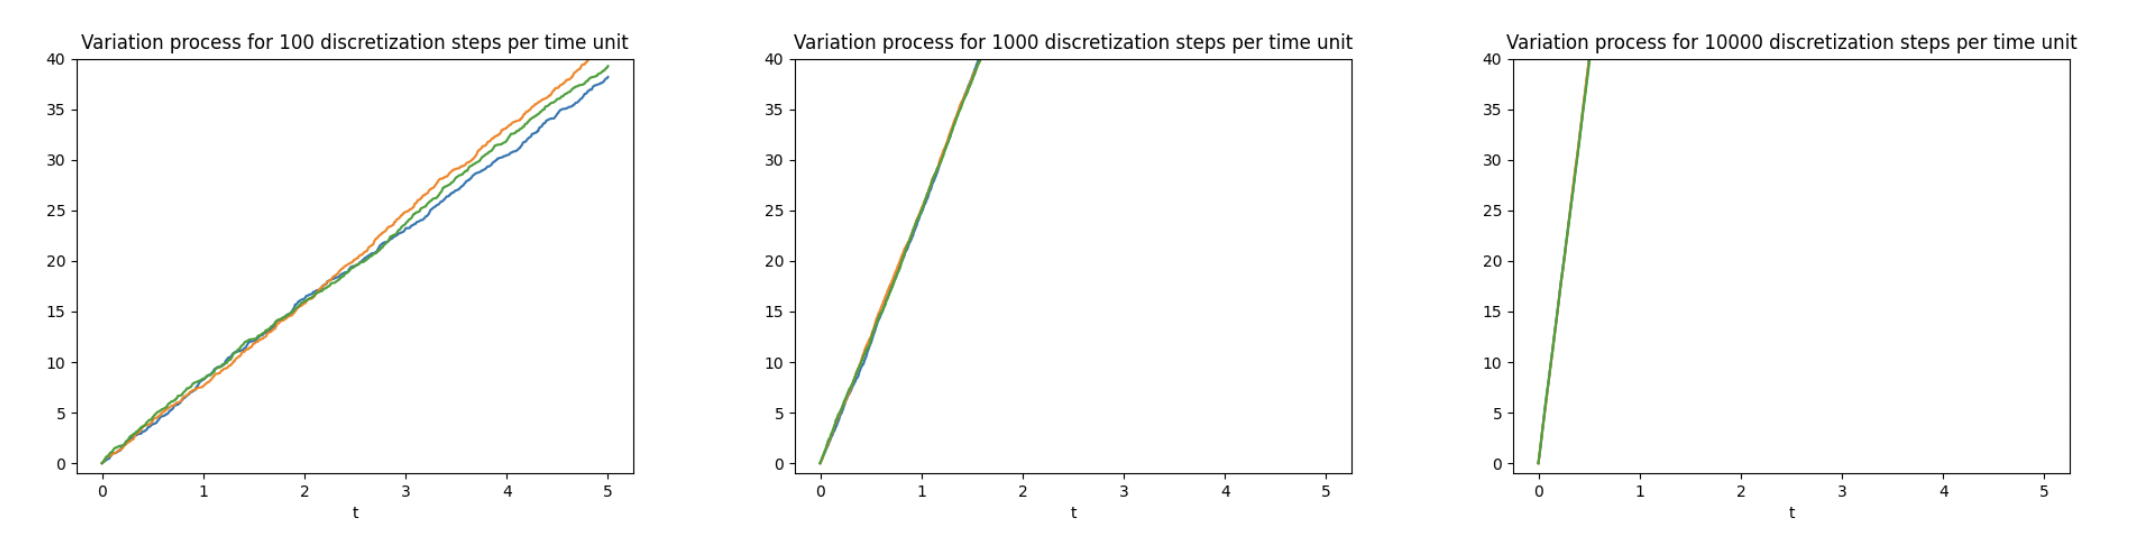
\includegraphics[width=1\textwidth]{Bilder/1.png}
\end{figure}
\begin{figure}[h]
    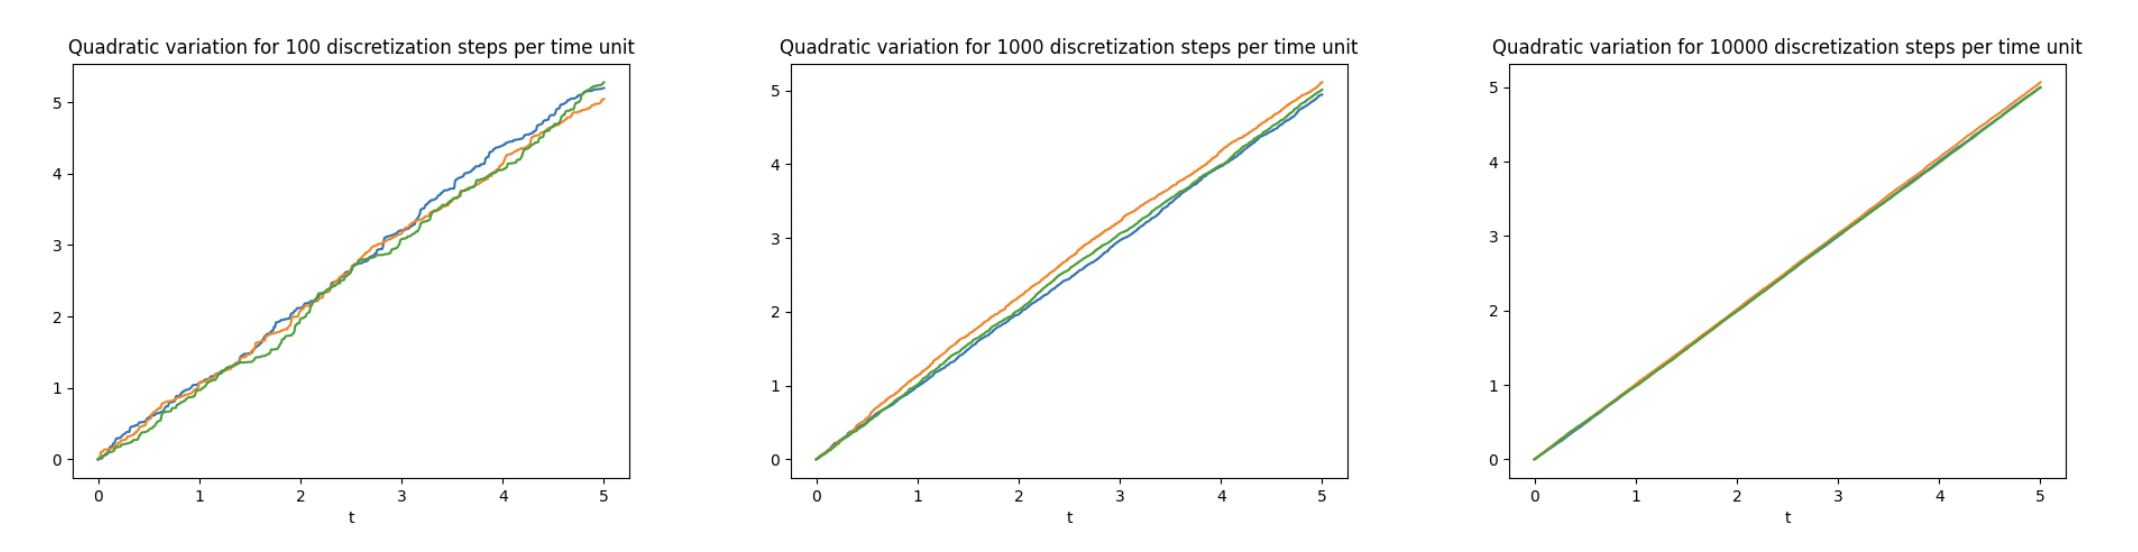
\includegraphics[width=1\textwidth]{Bilder/2.png} 
\end{figure}
\end{minipage}
\end{frame}


\begin{frame}{Einfache Ito Integral}
Für einfache Prozesse $(f_n(\cdot,t))_{t \geq 0}$, d.h. der form
\[
f_n (\cdot,t) := \sum_{i=1}^{n-1} X_i, \textbf{1}_{(t_i,t_{i+1}]} (t), \quad X_i \in L^2( (\Omega,\mathcal{F}_{t_i}, \mathbb{P}); \mathbb{R}^d )
\]
definieren wir das einfache Ito Integral 
\[
I(f(\cdot,\cdot))_t := \sum_{i=1}^{n-1} X_i (W_{t_{i+1} \wedge t} - W_{t_i \wedge t}), \quad t \in [0,T].
\]
\end{frame}

\begin{frame}{Integranten des Ito Integrals}
Man kann zeigen, dass
\[
\mathbb{E}[ \int_0^T f^2(\cdot,s) ds ]= \mathbb{E}[ \int_0^T f^2(\cdot,s) d\langle W \rangle_s ] = \mathbb{E}[ \left(\int_0^T f(\cdot,s) dW_s \right)^2 ].
\]
Wir definieren, das Ito Integral (prozess) auf der Menge der Zulässigen integranten: Funktionen in $L^2( \Omega \times [0,T], \mathbb{P} \otimes \lambda )$ und noch ein paar Eigenschaften erfüllen: 
\[
\mathcal{L}_T := \{ f: \Omega \times [0,T] \to \mathbb{R} \mid f \text{ messbar, adaptiert und } \mathbb{E}[ \int_0^T f^2(\cdot,s) ds ]<\infty \}. 
\]
\end{frame}

\begin{frame}{Ito Integral}
\begin{block}{Existenz}
  Für jedes $f \in \mathcal{L}_T$ existiert $( (f_n(\cdot,t))_{t \geq 0} )_{n \in \mathbb{N}}$ sodass 
  \[
  \| f_n - f \|_{\mathcal{L}_T} \to 0, \quad n\to \infty.
  \]
\end{block}
Das Ito Integral für $(f(\cdot,t))_{t \geq 0}$ ist damit der Grenzwert des einfaches Ito Integrals 
\[
\int_0^t f(\cdot,t) dW_t := \mathcal{L}_T - \lim_{n \to \infty} I(f_n(\cdot,\cdot))_t.
\]
\end{frame}





\subsection{Starke Lösungen von Stochastische Differentialgleichungen}

\begin{frame}{Stochastische Differentialgleichung}
Seien $b: \mathbb{R}^n \to \mathbb{R}^n$ und $\sigma: \mathbb{R}^n \to \mathbb{R}^{n \times m}$, dann nennen wir den stochastischen Prozess $(X_t)_{t \in [0,T]}$ mit stetigen Pfaden \textbf{starke}-Lösung der SDE 
\[
d X_t = b (X_t) dt + \sigma (X_t) d W_t, \quad t \in [0,T], \quad X_0 =x_0 \in \mathbb{R}^n,
\]
falls \\

\begin{minipage}[c]{0.30\linewidth}{\tiny
  \begin{itemize}
    \item $(X_t)_{t \in [0,T]}$ ist $(\mathcal{F}_t)_{t \in [0,T]}$ adaptiert
    \item $\mathbb{P}(X_0 =x_0) =1$
  \end{itemize}}
\end{minipage}\hfill
\begin{minipage}[c]{0.70\linewidth}{\tiny
\begin{itemize}
  \item $
        \forall i=1,...,d, j=1,...,r \text{ und } t \in [0,\infty): \quad \mathbb{P}(\int_0^t |a_i (s,X_s)| + b_{ij}^2 (s,X_s) ds < \infty)=1
        $
        \item 
        $
        \forall t \in [0,T], i=1,...,d: \quad X_t^{i} = X_0^{i} + \int_0^t a_i (s,X_s) ds + \sum_{j=1}^r \int_0^t b_{ij} (s,X_s) dW_s^j \quad \mathbb{P}-f.s.
        $
\end{itemize}
}
\end{minipage}
\end{frame}

\begin{frame}{Existenz der Starke Lösung}

  \begin{block}{Existenz}
    Für $b : \mathbb{R}^n \to \mathbb{R}^n$ und $\sigma: \mathbb{R}^n \to \mathbb{R}^{n\times m}$ mit  
    \[
    \exists C>0 \forall x,y \in \mathbb{R}^n: \substack{ |b(x)-b(y)|^2 + |\sigma (x) - \sigma(y)|^2 \leq C |x-y|^2 \\ |b(x)|^2 + |\sigma (x)|^2 \leq C(1+|x|^2)}
    \]
    existiert eine eindeutige starke Lösung der SDE in $X \in \mathcal{L}_T$, d.h. für eine weitere starke Lösung $Y \in \mathcal{L}_T$ gilt 
    \[
    \mathbb{P} (X_t = Y_t, t \in [0,T]) =1.
    \]
  \end{block}
\end{frame}

\begin{frame}{Hauptsatz Integralrechnung für Ito Integrale}\small
  Der Hauptsatz der Integralrechnung aus der Analysis gibt es auch für Ito Integrale. Eine vereinfachte Version mit $n=m=1$ ist: 
 \begin{block}{Ito Formel}
  Für $F \in C^2(\mathbb{R};\mathbb{R})$ und es gibt $C>0 , p \geq 1$ sodass 
  \[
  \forall x \in \mathbb{R}^n: \quad |F(x)| + |F^\prime (x)| \leq C (1+ |x|^p),
  \]
  und $X$ Lösung der SDE, dann gilt 
  \[
  F(X_t) - F(X_0) = \int_0^t F^\prime (X_s) a(X_s) ds + \underbrace{ \int_0^t F^\prime (X_s) \sigma (X_s) d W_s + \frac{1}{2} \int_0^t F^{\prime \prime} (X_s) |\sigma (X_s)|^2 ds }_{Neu} \quad \mathbb{P}-f.s.
  \]
   \end{block}
\end{frame}

\begin{frame}{Girsanov Theorem}
  Für das Martingal 
  \[
  L:= \left( L_t := \exp \left( \int_0^t X_s dW_s - \frac{1}{2} \int_0^t X_s^2 ds  \right)  \right)_{t \in [0,T]},
  \]
  auf $(\Omega,\mathcal{F}_T, \mathbb{P})$ bzgl. der Brownschen Filtration, d.h. $\left( \mathcal{F}_t := \sigma (W_s : s \leq t) \right)_{t \in [0,T]}$ ist für $\tilde{W}_t := W_t - \int_0^t X_s ds$ der Prozess $\tilde{W} := (\tilde{W}_t)_{t \geq 0}$ eine Brownsche Bewegung auf $(\Omega,\mathcal{F}_T,(\mathcal{F}_t)_{t \in [0,T]}, Q)$, wobei 

\begin{minipage}[c]{0.40\linewidth}{
\[
  \frac{d}{d\mathbb{P}} Q = L_T.
  \]
}
\end{minipage}\hfill
\begin{minipage}[c]{0.60\linewidth}
\recallbox[Radon-Nikodym:]{\small
$ \forall A \in \mathcal{F}_T: \quad \int_A d Q = \int_A \frac{d}{d\mathbb{P}} Q d \mathbb{P} $.
}
\end{minipage}
\end{frame}


\section{Partielle Differentialgleichungen}
\begin{frame}{Gewöhnliche Differentialgleichung}

\begin{minipage}[c]{0.60\linewidth}
   \begin{block}{Anfangswertproblem}
    Sei $f: U \subset \mathbb{R}^2 \to \mathbb{R}$ and $(\xi,\eta) \in U$. Eine differenzierbare Funktion $u: I \subset \mathbb{R} \to \mathbb{R}$ mit $\xi \in I$ nennt man Lösung des Anfangswertproblems, falls 
    \begin{align*}
    \forall t \in I: \frac{d}{dt} u(t) &= f(t,u(t)) \\ u(\xi) &= \eta .
    \end{align*}
    \end{block}
\end{minipage}\hfill
\begin{minipage}[c]{0.40\linewidth}
\begin{figure}[h]
    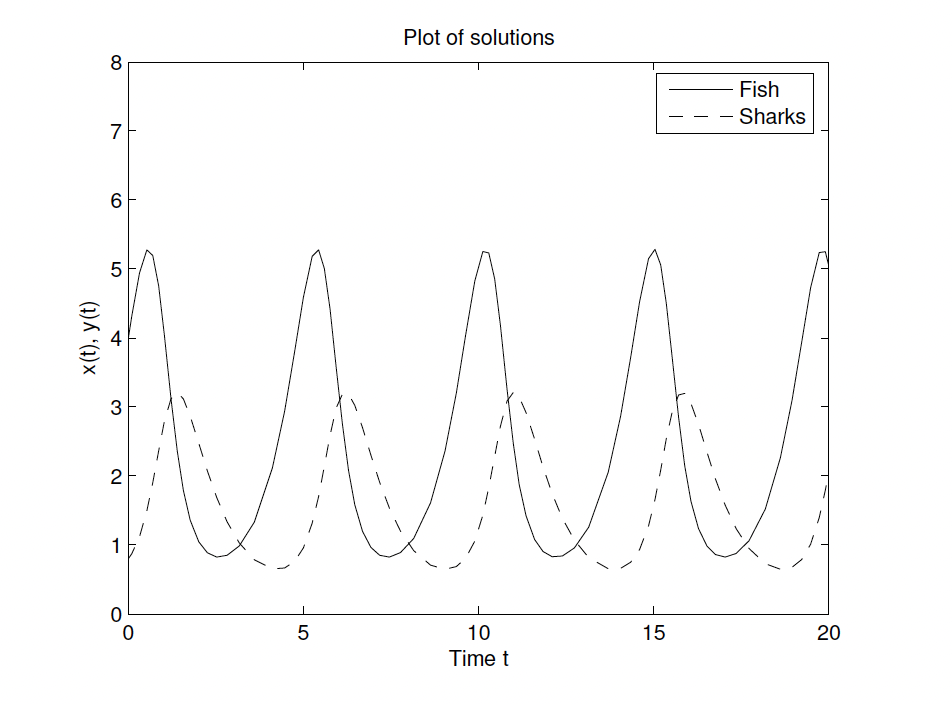
\includegraphics[width=0.6\textwidth]{Bilder/5.png}
\end{figure}
\begin{figure}[h]
    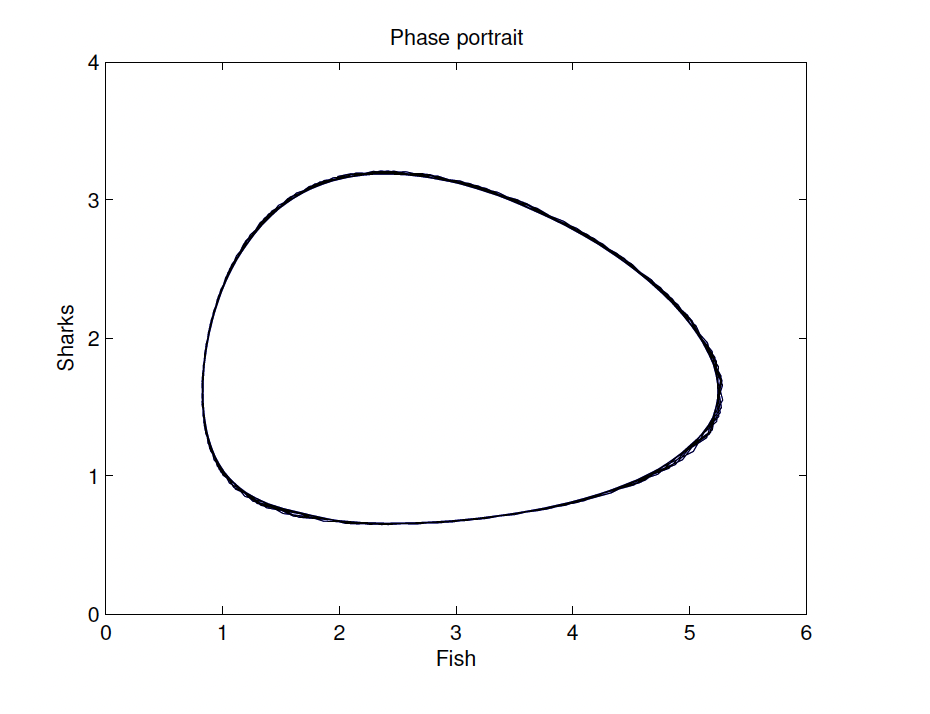
\includegraphics[width=0.6\textwidth]{Bilder/6.png} 
\end{figure}
\end{minipage}
\end{frame}




\begin{frame}{Differential Operatoren}
\begin{block}{Differential Operator} 
  Für offene und verbundene Teilmengen $A \subset \mathbb{R}^n$ nennen wir den linearen Operator 
  \begin{align*}
  &L: C^2(A) \to C^0 (A), u \mapsto (c\mapsto (Lu)(x)), \\
  &Lu:= -\sum_{i,j=1}^n a_{ij} (\cdot) \frac{\partial^2}{\partial x_i \partial x_j} u(\cdot) + \sum_{i=1}^n b_i (\cdot) \frac{\partial}{\partial x_i} u(\cdot) + c(\cdot) u(\cdot),
  \end{align*}
  Differential Operator.
\end{block}
\end{frame}

\begin{frame}{Differentialgleichungen}  \tiny
Eine Differentialgleichung zweiter Ordnung ist gegeben durch 
\[
\forall x \in A: \quad \frac{\partial}{\partial t} u(x,t)= (Lu(\cdot,t))(x)
\]
und $u \in C^2 (A \times [0,T]) \cap C^0 (A \times [0,T])$ nennt man klassische Lösung.

\centering
  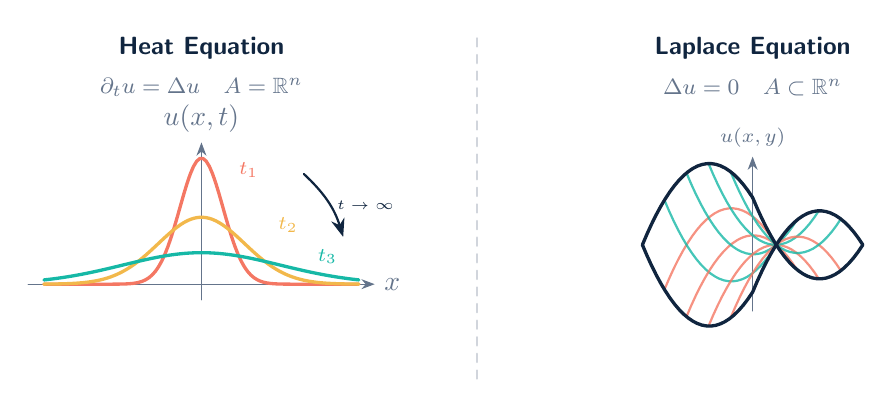
\begin{tikzpicture}[>=Stealth, line cap=round, line join=round]
    
    % --- LEFT: HEAT EQUATION (Dynamics / Evolution) ---
    \begin{scope}[xshift=-3.5cm]
      \node[font=\sffamily\small\bfseries, text=Midnight] at (0, 3.0) {Heat Equation};
      \node[font=\footnotesize, text=Muted] at (0, 2.5) {$\partial_t u = \Delta u \quad A=\mathbb{R}^n $};
      
      % Axes
      \draw[->, Muted, thin] (-2.2, 0) -- (2.2, 0) node[right] {$x$};
      \draw[->, Muted, thin] (0, -0.2) -- (0, 1.8) node[above] {$u(x,t)$};
      
      % Multiple time points of the fundamental solution (Gaussians)
      % t1 (sharp, early time)
      \draw[Coral, very thick, domain=-2:2, samples=100] plot (\x, {1.6*exp(-\x*\x/0.15)});
      \node[font=\scriptsize, text=Coral] at (0.6, 1.45) {$t_1$};
      
      % t2 (medium spread)
      \draw[Gold, very thick, domain=-2:2, samples=100] plot (\x, {0.85*exp(-\x*\x/0.6)});
      \node[font=\scriptsize, text=Gold] at (1.1, 0.75) {$t_2$};
      
      % t3 (wide, late time)
      \draw[Teal, very thick, domain=-2:2, samples=100] plot (\x, {0.4*exp(-\x*\x/2.0)});
      \node[font=\scriptsize, text=Teal] at (1.6, 0.35) {$t_3$};
      
      % Arrow indicating the flow of time
      \draw[->, Midnight, thick] (1.3, 1.4) to[bend left=15] (1.8, 0.6);
      \node[font=\tiny\bfseries, text=Midnight, right] at (1.6, 1.0) {$t \to \infty$};
      
     
    \end{scope}
    
    % --- RIGHT: LAPLACE EQUATION (Steady State / Equilibrium) ---
    \begin{scope}[xshift=3.5cm]
      \node[font=\sffamily\small\bfseries, text=Midnight] at (0, 3.0) {Laplace Equation};
      \node[font=\footnotesize, text=Muted] at (0, 2.5) {$\Delta u = 0 \quad  A\subset \mathbb{R}^n$};
      
      % 3D Scope for the Saddle/Membrane (z = x^2 - y^2)
      \begin{scope}[shift={(0,0.5)}, x={(0.7cm, -0.3cm)}, y={(0.7cm, 0.3cm)}, z={(0cm, 0.7cm)}]
        
        % Z-Axis
        \draw[->, Muted, thin] (0,0,-1.2) -- (0,0,1.6) node[above, font=\scriptsize] {$u(x,y)$};
        
        % Membrane Grid (orthogonal curvatures cancel each other out)
        \foreach \i in {-1, -0.6, -0.2, 0.2, 0.6, 1} {
           % x-constant lines
           \draw[Coral, thick, opacity=0.8] plot[domain=-1:1, samples=25] (\i, \x, {\i*\i - \x*\x});
           % y-constant lines
           \draw[Teal, thick, opacity=0.8] plot[domain=-1:1, samples=25] (\x, \i, {\x*\x - \i*\i});
        }
        
        % Fixed boundary (wireframe holding the membrane)
        \draw[Midnight, very thick] plot[domain=-1:1, samples=25] (1, \x, {1 - \x*\x});
        \draw[Midnight, very thick] plot[domain=-1:1, samples=25] (-1, \x, {1 - \x*\x});
        \draw[Midnight, very thick] plot[domain=-1:1, samples=25] (\x, 1, {\x*\x - 1});
        \draw[Midnight, very thick] plot[domain=-1:1, samples=25] (\x, -1, {\x*\x - 1});
        
      \end{scope}
      
     
    \end{scope}

    % Divider
    \draw[Muted!30, thick, dashed] (0, -1.2) -- (0, 3.2);

  \end{tikzpicture}


\end{frame}













\section{Markov Prozesse}
\begin{frame}{Markov Übergangsfunktion}
Eine Abbildung $P: [0,\infty) \times E \times \mathcal{E} \to [0,1]$ nennt man zeithomogene Markov Übergangsfunktion auf $(E,\mathcal{E})$, falls 
\begin{itemize}
  \item $\forall t \geq 0$: $P(t,\cdot,\cdot)$ ist Markovkern von $(E,\mathcal{E})$ nach $(E,\mathcal{E})$
  \item $\forall s,t \geq 0$: $P(s+t,\cdot,\cdot)= P(t,\cdot,\cdot)\circ P(s,\cdot,\cdot)$
\end{itemize}
\end{frame}


\begin{frame}{Halbgruppen}

  \begin{block}{Halbgruppe}
  Eine Familie $(P_t)_{t \geq 0}$ heißt Markov Halbgruppe, falls für alle $s,t \geq 0$: 

\begin{minipage}[c]{0.50\linewidth}
  \begin{itemize}
    \item $P_t: \mathcal{B}(E) \to \mathcal{B}(E)$ beschränkt
    \item $\forall f \in \mathcal{B}(E)$ mit $0\leq f \leq 1$: $0\leq P_t f \leq 1$
  \end{itemize}
\end{minipage}\hfill
\begin{minipage}[c]{0.50\linewidth}
\begin{itemize}
  \item $P_{t+s} =P_s \circ P_t$
  \item $\forall (f_n)_{n \in \mathbb{N}} \subseteq \mathcal{B}(E)$ mit $f_n \searrow 0$: $P_t f_n \searrow 0$.
\end{itemize}
\end{minipage}
\end{block}

\begin{block}{Markov Halbgruppe}
  Sei $P$ eine Markov Übergangsfunktion auf $(E,\mathcal{B}(E))$ dann ist 
  \[
  \forall f \in \mathcal{B}(E), x \in E, t \geq 0: \quad (P_t f) (x) := \int_E f(y) d (\mathbb{P}_x \circ X_t^{-1})(y),
  \]
  eine Markov Halbgruppe.

\end{block}


\end{frame}



\begin{frame}{Markovprozess}
Sei $(\Omega,\mathcal{F}, (\mathcal{F}_t)_{t \geq 0})$ ein filtrierter Raum, $(E,\mathcal{B}(E))$ ein polnischer Raum auf $(\Omega,\mathcal{F})$ und $(\mathbb{P}_x)_{x \in E}$ eine Familie von von Wahrscheinlichkeitsmaßen auf $(\Omega,\mathcal{F})$. Wir nennen $(X_t)_{t \geq 0}$ einen Markovprozess, falls 
\begin{itemize}
  \item $\forall B \in \mathcal{F}_\infty^X : x \mapsto \mathbb{P}_x (B)$ is $\mathcal{B}(E)$ messbar
  \item Die schwache Markoveigenschaft gilt 
  \[
  \forall x \in E, A \in \mathcal{B}(E), s,t \geq 0: \quad \mathbb{P}_x [ X_{t+s} \in A \mid \mathcal{F}_s ] = \mathbb{P}_{X_s} (X_t \in A), \quad \mathbb{P}_x-f.s.
  \]
\end{itemize}

\recallbox[]{\tiny
$P(t,\cdot,\cdot)$ Übergangsfkt. $\iff$ $(P_t)_{t \geq 0}$ Markov Halbgr. $\iff$ $X$ Markov Proz. $\iff$ ... $\iff$ ...
}
\end{frame}


\begin{frame}{Generatoren}
\begin{block}{Generator}
  Sei $(P_t)_{t \geq 0}$ eine Markov Halbgruppe auf $\mathcal{B}(E)$, dann heißt 
  \[
  G: \mathcal{D}(F):= \{ f \in \mathcal{B}(E) \mid s-\lim_{t \searrow 0} (P_t f-f) \text{ existiert} \} \subseteq B(\mathcal{E}) \to \mathcal{B}(E)
  \] 
  infitesimal generator von $(P_t)_{t \geq 0}$, falls 
  \[
  \forall f \in \mathcal{D}(G): \quad Gf= s-\lim_{t \searrow 0} (P_t f-f).
  \]
\end{block}
\end{frame}


\begin{frame}{Key Message}

  $P(t,\cdot,\cdot)$ Übergangsfkt. $\iff$ $(P_t)_{t \geq 0}$ Markov Halbgr. $\iff$ $X$ Markov Proz. $\iff$ $(G,\mathcal{D}(G))$ Generator
  
\end{frame}




\section{Rückwärts Prozesse}

\begin{frame}{Explodierende und Terminierende Prozesse und die Messbarkeit}
 
Ein stochastischer Prozess muss für alle $\omega \in \Omega$ wohl definiert sein. Wenn $(X_t)_{t \geq 0}$
\begin{itemize}
  \item nach endlicher Zeit explodiert oder 
  \item nach endlicher Zeit terminiert wird
\end{itemize} 
ist $(X_t)_{t \geq 0}$ nicht mehr messbar! Sei $\Delta$ der Zustand, den der Proess annimmt, wenn er explodiert oder terminiert wird. Betrachte $E_\Delta := E \cup \Delta$ und 
\[
\zeta (\omega) := \inf \{ t \geq 0 \mid X_t(\omega) = \Delta \}
\]
Eintrittszeit von $\Delta$.
\end{frame}


\begin{frame}{Problem der Stoppzeit}\tiny
Sei $T: \Omega \to \mathbb{N}\cup \{\infty \}$ eine Stoppzeit bzw. erste Eintrittszeit von  $A \in \mathcal{F}$ und $\theta_u : \Omega \to \Omega, \omega \mapsto (\theta_u \omega)(\cdot) := \omega (u+\cdot)$ Verschiebungsoperator, dann gilt 
\begin{align*}
T(\theta_t \omega) = \inf \{ s\geq 0 \mid X_{t+s} (\omega)\in A \} = \inf \left( \underbrace{\{ s \geq 0 \mid X_s (\omega)\in A \}}_{=:S} \cap [0,\infty) \right) -t = \inf \{ s \geq t \mid X_s (\omega) \in A \}-t =: D_t -t.
\end{align*}
\begin{itemize}
  \item Fall $\omega \in \{ T \geq t \}$: 
  \[
  T(\theta_t \omega) = \inf \left( \underbrace{S}_{\subseteq [T,\infty) \subseteq [t,\infty) } \cap [t,\infty) \right) -t = \inf (S) -t = T(\omega) -t.
  \]
  Wir können Stoppzeiten bzgl. der Vergangheit verschieben.
  \item Fall $\omega \in \{ T < t \}$:
  \[
  D_t (\omega) \geq t \quad \implies \quad T \circ \theta_t = D_t -t \geq 0 = (T-t)_+.
  \]
  Wir können Stoppzeiten nicht bzgl. der Zukunft verschieben!
\end{itemize}
\end{frame}

\begin{frame}{Lösung des Problems}
  
  \begin{block}{Ko-Optionale Zeiten}
    Eine Zufallsvariable $L: \Omega \to \mathbb{R}^+$, falls 
    \begin{itemize}
      \item $\{L< \infty \} \subseteq \{L< \zeta\}$
      \item $\forall t \geq 0:$ $L \circ \theta_T = (T-t)_+$.
    \end{itemize}
  \end{block}
\end{frame}


\begin{frame}{Rückwärts Prozess}

Der Rückwärtsprozess ist definiert als 
\[
\forall t \geq 0: \quad \bar{X}_t (\omega) := \begin{cases}
  \Delta &, L(\omega) \leq t \vee L(\omega) =\infty \\
  X_{L(\omega)-t} (\omega) &, t \in (0,L(\omega))
\end{cases}, \quad \bar{X}_0 := \begin{cases}
  X_{L-} &, L \in (0,\infty)\\
  \Delta &\text{sonst}
\end{cases}
\]
und die Rückwärtsfiltration $\bar{\mathcal{F}}_t := \sigma (\bar{X}_s : s \leq t)$.
\end{frame}

\begin{frame}{Von Reversibilität zur Markoveigenschaft (1/2)}

\begin{block}{Reversibilität}
Sei $(P_t)_{t \geq 0}$ eine halb-Gruppe eines Markov Prozesses. Wir nenn ihn reversibel bzgl. dem Wahrscheinlichkeitsmaß $\nu$, falls alle $P_t$ selbstadjungiert sind im Hilbertraum $L^2(E,\nu)$, d.h. 
\[
\forall t \geq 0, f,g \in L^2(E,\nu): \quad \langle P_t f,g \rangle_\nu := \int_E (P_t f) g d \nu = \int_E f (P_t g) d \nu = \langle f,P_t g \rangle_\nu.
\]  
\end{block}
Die Brownsche Bewegung $(W_t)_{t \geq 0}$ ist reversibel, da der Generator $\frac{1}{2} \Delta$ selbstadjungiert ist in $L^2(E,\nu)$: 
\[
\langle \Delta f,g \rangle= \int_E \Delta f g d \nu = \int_E f \Delta g d \nu = \langle f,\Delta g \rangle.
\]
\end{frame}

\begin{frame}{Von Reversibilität zur Markoveigenschaft (2/2)}

  \[
  \forall A \in \bar{\mathcal{F}}_t: \quad A \cap \{ L \cap \{ L > t+u \} = \theta_u^{-1} (A \cap \{ L> t \}),
  \]
  dann 
  \[
  \mathbb{P}( A \cap \{ L> t+ u \} \mid \mathcal{F}_u ) = \mathbb{P}( \theta_u^{-1} ( A \cap \{L>t+u\}) \mid \mathcal{F}_u) =\mathbb{P}_{X_u} (A \cap \{L> t+u\}).
  \]

\end{frame}



\section{Zusammenführung von SDEs und PDEs}

\begin{frame}{Von SDEs zu PDEs}\tiny
Sei $\phi \in C_c^\infty ( \mathbb{R}^d \times [0,T])$ beliebig, $X$ eine Lösung der SDE, wobei die marginale dichte von $X_t$ gegeben ist durch $p(\cdot,t)$ und $a:= \sigma^T \sigma$, dann gilt 
\begin{align*}
    0= \mathbb{E}[ \phi(X_T,T)- \phi(X_0,0) ]&\stackrel{Ito-Formel}{=} \mathbb{E}[ \int_0^T \frac{\partial}{\partial s} \phi (X_s,s)+\nabla \phi (X_s,s) b(X_s,s) + \Delta \phi (X_s,s) a(X_s,s)ds  ] \\
    &+ \underbrace{\mathbb{E}[ \int_0^T \nabla \phi (X_s,s) \sigma(X_s,s)d W_s ]}_{=0, \text{ Integralprozess ist Martingal}}\\
    &= \int_0^T \int_{\mathbb{R}^n} \left( \frac{\partial}{\partial s} \phi (x,s) + b(x,s)^T \nabla \phi (x,s) + \Delta \phi (x,s) \right) p(x,s) dx ds\\
    &=\int_0^T \int_{\mathbb{R}^n} \left(- \frac{\partial}{\partial s} p (x,s) -\nabla \cdot ( p(x,s) b(x,s))   + \Delta p (x,s) \right) \phi (x,s) dx ds 
\end{align*}
Man sagt, $p$ löst die Differentialgleichung $\frac{\partial}{\partial t} p (x,t) + \nabla \cdot ( p(x,t) b(x,t)) = \Delta p(x,t)$ im schwachen Sine.
\end{frame}

\begin{frame}{Die SDE und PDE für den Rückwärtsprozess}\tiny
Auf ähnliche Art und Weise kann man für Testfunktionen $\psi (x,t) := \phi (x,T-t)$ zeigen, dass 
\begin{align*}
0&=  \int_0^T \int_{\mathbb{R}^n}- \frac{\partial}{\partial s} \bar{u}(x,s) \psi (x,s) + \nabla \cdot( b(x,T-s) \bar{u}(x,s)) \psi(x,s)+\Delta \bar{u}(x,s) \psi(x,s) \\
&- 2 \nabla \cdot ( \bar{u}(x,s) \nabla \log( \bar{u}(x,s)))  \psi (x,s)   dx ds.
\end{align*}
Dies ist äquivalent zu 
\[
-\frac{\partial}{\partial t} \bar{u} + \nabla \cdot ( b(\cdot,T-\cdot) \bar{u} ) + \Delta \bar{u} - 2 \nabla \cdot ( \bar{u} \nabla \log (\bar{u}))=0 \quad \iff \quad 
\frac{\partial}{\partial t} \bar{u} = - \Delta \bar{u} + \nabla \cdot ( b(\cdot,T-\cdot) \bar{u} ),
\]
was uns die SDE gibt: 
\[
d\bar{X}_t = \underbrace{(-b(\bar{X_t}+ \sigma(\bar{X}_t)^2 \nabla \log(p(T-t,\bar{X}_t) )}_{=: \bar{b}(\bar{X}_t)} dt + \sigma(\bar{X}_t) d \tilde{W}_{t}, \quad X_t \sim \bar{p}(\cdot,t), 
\]

\end{frame}


\begin{frame}{Wo stehen wir jetzt und was ist das Problem?}
  \textbf{Problem}: Die PDE explodiert nach endlicher Zeit und der Drift der SDE ist nicht Lipschitzstetig! \textbf{Wir brauchen einen neuen Lösungsbegriff!}
  \[
  \frac{\partial}{\partial t} \bar{u} = - \Delta \bar{u} + \nabla \cdot ( b(\cdot,T-\cdot) \bar{u} ),
  \]
  und
  \[
d\bar{X}_t = \underbrace{(-b(\bar{X_t}+ \sigma(\bar{X}_t)^2 \nabla \log(p(T-t,\bar{X}_t) )}_{=: \bar{b}(\bar{X}_t)} dt + \sigma(\bar{X}_t) d \tilde{W}_{t}, \quad X_t \sim \bar{p}(\cdot,t), 
\]
\end{frame}


\section{Schwache Formulierungen}




\subsection{Schwache Formulierung von Partiellen Differentialgleichungen}

\begin{frame}{Distributionen}
  Für $A \subseteq \mathbb{R}^n$ ist der Lineare operator 
\[
\langle \partial_i f, \cdot \rangle : \mathcal{D}(A) \to \mathbb{R}, \quad \phi \mapsto \langle \partial_i f , \phi \rangle :=- \langle f, \partial_i \phi \rangle
\]
eine Distribution und heißt schwache Ableitung. Eine schwache Lösung der PDE $\partial_t u = L u$ ist definiert als die Lösung $u: A \to \mathbb{R}$ sodass 
\[
\forall \phi \in C_0^\infty (A): \langle \partial_t u, \phi \rangle = -\int_s^t \int_{\mathbb{R}^n} u (x,z) \partial_t \phi (x,z) dx dz = -\int_s^t \int_{\mathbb{R}^n} u(x,z) L_z \phi (x,z) dx dz = \langle L u , \phi \rangle 
\]
\end{frame}





\begin{frame}{Regularität: Stark vs. Schwache Lösungen}
  \centering
  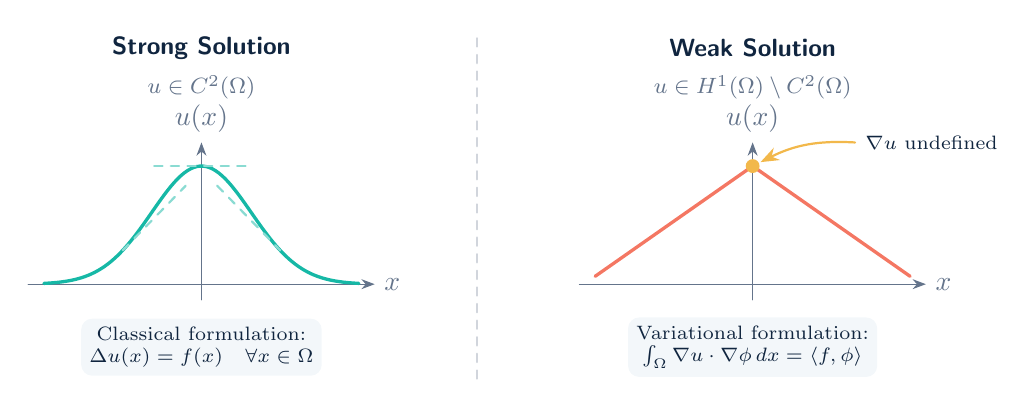
\begin{tikzpicture}[>=Stealth, line cap=round, line join=round]
    
    % --- LEFT: STRONG SOLUTION ---
    \begin{scope}[xshift=-3.5cm]
      % Überschriften nach oben verschoben (y=3.0 und y=2.5)
      \node[font=\sffamily\small\bfseries, text=Midnight] at (0, 3.0) {Strong Solution};
      \node[font=\footnotesize, text=Muted] at (0, 2.5) {$u \in C^2(\Omega)$};
      
      % Coordinate system
      \draw[->, Muted, thin] (-2.2, 0) -- (2.2, 0) node[right] {$x$};
      \draw[->, Muted, thin] (0, -0.2) -- (0, 1.8) node[above] {$u(x)$};
      
      % Smooth curve (e.g., Gaussian/Bell curve representing C^2 solution)
      \draw[Teal, very thick, domain=-2:2, samples=100] plot (\x, {1.5*exp(-\x*\x/0.8)});
      
      % Tangent lines to show continuous first derivative
      \draw[Teal!50!white, thick, dashed] (-1, 0.43) -- (-0.2, 1.25);
      \draw[Teal!50!white, thick, dashed] (0.2, 1.25) -- (1, 0.43);
      \draw[Teal!50!white, thick, dashed] (-0.6, 1.5) -- (0.6, 1.5);
      
      % Math label
      \node[font=\scriptsize, text=Midnight, align=center, fill=Mist, rounded corners, inner sep=3pt] 
        at (0, -0.8) {Classical formulation:\\$\Delta u(x) = f(x) \quad \forall x \in \Omega$};
    \end{scope}
    
    % --- RIGHT: WEAK SOLUTION ---
    \begin{scope}[xshift=3.5cm]
      % Überschriften nach oben verschoben (y=3.0 und y=2.5)
      \node[font=\sffamily\small\bfseries, text=Midnight] at (0, 3.0) {Weak Solution};
      \node[font=\footnotesize, text=Muted] at (0, 2.5) {$u \in H^1(\Omega) \setminus C^2(\Omega)$};
      
      % Coordinate system
      \draw[->, Muted, thin] (-2.2, 0) -- (2.2, 0) node[right] {$x$};
      \draw[->, Muted, thin] (0, -0.2) -- (0, 1.8) node[above] {$u(x)$};
      
      % Tent function (representing H^1 solution with a point singularity)
      \draw[Coral, very thick] (-2, 0.1) -- (0, 1.5) -- (2, 0.1);
      
      % Highlighting the kink (non-differentiable point)
      \fill[Gold] (0, 1.5) circle (2.5pt);
      \draw[->, Gold, thick] (1.3, 1.8) node[right, font=\scriptsize, text=Midnight] {$\nabla u$ undefined} to[bend right=15] (0.1, 1.55);
      
      % Math label
      \node[font=\scriptsize, text=Midnight, align=center, fill=Mist, rounded corners, inner sep=3pt] 
        at (0, -0.8) {Variational formulation:\\$\int_\Omega \nabla u \cdot \nabla \phi \, dx = \langle f, \phi \rangle$};
    \end{scope}

    % Trennlinie (nach oben verlängert, um den neuen Abstand auszufüllen)
    \draw[Muted!30, thick, dashed] (0, -1.2) -- (0, 3.2);

  \end{tikzpicture}
\end{frame}





\subsection{Schwache Formulierung von Stochastische Differentialgleichungen}



\begin{frame}{Schwache Lösung der SDE}
  Eine schwaceh Lösung der mit Startverteilung $\mu$ auf $\mathcal{B}(\mathbb{R}^d)$ von 
    \[
    dX_t = b(t,X_t) dt + \sigma (t,X_t) dW_t
    \]
    ist ein Tupel $((\Omega,\mathcal{F},\mathbb{P}), (\mathcal{F}_t)_{t \geq 0}, X, W)$ wobei $(\Omega,\mathcal{F},(\mathcal{F}_t)_{t \geq 0}, \mathbb{P})$ ein filtrierter Wahrscheinlichkeitsraum ist, wobei die Filtration die üblichen Bedinungen erfüllt, $X$ ist $(\mathcal{F}_t)$-adaptiert, $\mathbb{R}^d$ wertiger Prozess und $W$ ein $r$-dimensionale $(\mathcal{F}_t)$-Brownsche Bewegung $W$
    \begin{itemize}
        \item 
        \[
        \forall i=1,...,d, j=1,...,r \text{ und } t \in [0,\infty): \quad \mathbb{P}(\int_0^t |a_i (s,X_s)| + b_{ij}^2 (s,X_s) ds < \infty)=1
        \]
        \item 
        \[
        \forall t \in [0,T], i=1,...,d: \quad X_t^{i} = X_0^{i} + \int_0^t a_i (s,X_s) ds + \sum_{j=1}^r \int_0^t b_{ij} (s,X_s) dW_s^j.
        \]
    \end{itemize}
\end{frame}

\begin{frame}{Filtrationen nicht fest gewählt}
  Further, the randomness in a strong solution only comes from
the randomness of the augmented standard Brownian filtration, whereas the randomness in a weak
solution comes from any filtration, with the restriction that W has to be a (Ft)-Brownian motion.
This means, that the solution at time t can not only be given by the initial condition, a measurable
functional given by the Brownian path and th
\end{frame}




\section{Martingale Problem}

\begin{frame}{Martingale Problem}

   Assume $b_i,\sigma_{ij}: \mathbb{R}^d \to \mathbb{R}$, $i=1,...,d, j=1,...,r$ are bounded on compact subsets of $\mathbb{R}^d$. We call a proability measure $\mathbb{P}$ on $(C([0,\infty)^d ), \mathcal{B}( C([0,\infty)^d) ) )$ under which for all $s,t \in [0,\infty), s<t, f \in C_0^2(\mathbb{R}^d)$: 
    \[
    \mathbb{E}[ f(y(t)) - f(y(0)) - \int_0^t (\mathcal{A}f)(y(u)) du \mid \mathcal{B}_s ] =0, \quad \mathbb{P}-a.s.
    \]
    a solution of the time-homogenous martingale problem. We denote by $\mathbb{P}^x$ any solution to this problem if it satisfies 
    \[
    \mathbb{P}^x (y \in C([0,\infty)^d ), y (0) =x)=1.
    \]
    The time-homogenous martingale problem is well posed if for every $x \in \mathbb{R}^d$, there is exactly one solution $\mathbb{P}^x$.

\recallbox[]{\tiny
 $(\mathbb{P}_x)_{x \in E}$ Wohlg. Mart. Probl. $\iff$ $(G,\mathcal{D}(G))$ Gen.
}
\end{frame}




\begin{frame}{Markov Eigenschaft der schwachen Lösung}
  Suppose the coefficients $b$ and $\sigma$ are bounded on compact subsets of $\mathbb{R}^d$ and the time-homogenous martingale problem is well posed. Then for every $\mathcal{B}_t$-stopping time $T$, $F \in \mathcal{B}(C([0,\infty)^d))$ and $x \in \mathbb{R}^d$: 
    \[
    \mathbb{P}^x[ \theta_T^{-1} (F) \mid \mathcal{B}_T ](\omega) = \mathbb{P}^{\omega(T)} (F), \quad \mathbb{P}^x-a.s. \text{ on } \{ T < \infty \}.
    \]
\end{frame}

\begin{frame}
  Let $b_i,\sigma_{ij}: \mathbb{R}^d \to \mathbb{R}$ be bounded and continuous and the time-homogenous SDE 
    \[
    dX_t = b(X_t) dt + \sigma (X_t)dW_t.
    \]
    For every initial distribution $\mu$ on $\mathcal{B}(\mathbb{R}^d)$ such that 
    \[
    \exists m>1: \quad \int_{\mathbb{R}^d} \| x \|^{2m} d \mu (x)< \infty,
    \]
    exists a weak solution. 
\end{frame}

\begin{frame}{Existenz }
   Let $\mathbb{P}$ be a probability measure on $(C([0,\infty)^d ), \mathcal{B}(C([0,\infty)^d))$ under which the process $M^f$ is a continuous local $\mathcal{F}_t$-martingale where $f(x) =x_i$ or $f(x) =x_i x_k$ for $i,k =1,...,d$. Then there exists a Brownian motion $W$ wrt. $(\tilde{\mathcal{F}}_t)_{t \geq 0}$ defined on the extension $(\tilde{\Omega},\tilde{\mathcal{F}}, \tilde{\mathbb{P}})$ of $(C([0,\infty)),\mathcal{B}(C([0,\infty)^d)),\mathbb{P})$ such that $((X_t := y(t),W_t),(\tilde{\Omega},\tilde{\mathcal{F}},\tilde{\mathbb{P}}),(\tilde{\mathcal{F}}_t))$ is a weak solution to the functional SDE.
\end{frame}


\begin{frame}{Martingale Problem und Starke Markov Eigenschaft}


\recallbox[]{\tiny
$P(t,\cdot,\cdot)$ Übergangsfkt. $\iff$ $(P_t)_{t \geq 0}$ Markov Halbgr. $\iff$ $X$ Markov Proz. $\iff$ $(\mathbb{P}_x)_{x \in E}$ Wohlg. Mart. Probl. $\iff$ $(G,\mathcal{D}(G))$ Gen.
}
\end{frame}


\begin{frame}{.}
.
\noindent
\begin{minipage}[c]{0.52\linewidth}
...
\end{minipage}\hfill
\begin{minipage}[c]{0.42\linewidth}

\end{minipage}
\end{frame}



\section{Anwendung zu Diffusion}
\begin{frame}{Recap und Problemstellung}
  Betrachte die SDE $dX_t = b(X_t,t) dt + \sigma(X_t,t) d W_t$.
\begin{itemize}
        \item $b: [0,1] \times \mathbb{R}^n \to \mathbb{R}^n$, $\sigma: [0,1] \times \mathbb{R}^n \to \mathbb{R}^n \otimes \mathbb{R}^l$ are borel measurable and satisfy 
        \begin{align*}
            |b(x,t) - b(y,t)| + |\sigma (x,t) - \sigma (y,t)| &\leq K |x-y|\\
            |b(x,t)| + | \sigma (x,t)| &\leq K(1+|x|),
        \end{align*}
        for some constant $K$.
        \item For $\lambda$-a.e. $t >0$,, $X_t \sim p(t,\cdot)$ such that $\forall t_0>0$: 
        \[
        p \in L^2( t_0,1; \tilde{H}_{loc}^1 ).
        \]
    \end{itemize}
\end{frame}


\begin{frame}{Beweis}
Problem: Der Drift vom Rückwärtsprozesses 
\[
\bar{b}(x,t) := -b(\bar{X}_t)  + \sigma(\bar{X}_t)^2 \nabla \log (p(T-t,\bar{X}_t)),
\]
ist nicht beschränkt auf kompakten teilmengen von $\mathbb{R}^n$! D.h. keine stetige Pfade! Martingal Problem vom Rückwärtsprozess bzgl. Rückwärtsgenerator $\bar{L}_z$ würde die Voraussetzungen nicht erfüllen!\\
Trick: Schreibe das Martingalproblem um, sodass es vom forwärts prozess abhängt bzgl. einem neuen generator.
\end{frame}

\begin{frame}{Markovprozess}
\begin{block}{Satz}
Angenommen
\begin{itemize}
        \item $b: [0,1] \times \mathbb{R}^n \to \mathbb{R}^n$, $\sigma: [0,1] \times \mathbb{R}^n \to \mathbb{R}^n \otimes \mathbb{R}^l$ are borel measurable and satisfy 
        \begin{align*}
            |b(x,t) - b(y,t)| + |\sigma (x,t) - \sigma (y,t)| &\leq K |x-y|\\
            |b(x,t)| + | \sigma (x,t)| &\leq K(1+|x|),
        \end{align*}
        for some constant $K$.
        \item For $\lambda$-a.e. $t >0$,, $X_t \sim p(t,\cdot)$ such that $\forall t_0>0$: 
        \[
        p \in L^2( t_0,1; \tilde{H}_{loc}^1 ),
        \]
    \end{itemize}
    dann ist $(\bar{X}_t)_{t \geq 0}$ ein Markov prozess mit generator 
    \[
    \bar{L}_t f:= \sum_{i,j=1}^n \frac{1}{2} a_{ij} (x,1-t) \frac{\partial^2}{\partial x_i \partial x_j} f(x)+ \sum_{i=1}^n (-b_i (x,1-t) + p(x,1-t)^{-1} \frac{\partial}{\partial x_j} (a_{ij} (x,1-t) p(x,1-t)) ) \frac{\partial}{\partial x_i} f(x) + 
    \]
\end{block}
\end{frame}

\begin{frame}{Problem}
Beliebige Testfunktionen: $f,g \in C_c^\infty(\mathbb{R}^n)$ und zeige für $0 \leq s < t < 1$: 
    \[
    \mathbb{E}[ f(\bar{X}_t)- f(\bar{X}_s)- \int_s^t (\bar{L}_z f)(\bar{X}_z) dz \mid \sigma (\bar{X}_r : 0 \leq r \leq s) ]=0.
    \]
    Weil $(\bar{X}_t)_{t \in [0,1)}$ Markov Prozess
    \begin{align*}
        \mathbb{E}[ f(\bar{X}_t)- f(\bar{X}_s)- \int_s^t (\bar{L}_z f)(\bar{X}_z) dz \mid \sigma (\bar{X}_r : 0 \leq r \leq s) ] &= \mathbb{E}[ f(\bar{X}_t)- f(\bar{X}_s)- \int_s^t (\bar{L}_z f)(\bar{X}_z) dz \mid \bar{X}_s] \\
        &= \mathbb{E}[ \left(f(\bar{X}_t)- f(\bar{X}_s)- \int_s^t (\bar{L}_z f)(\bar{X}_z) dz  \right) g(\bar{X}_s)] =0.
    \end{align*}
    Man kann zeigen, dass dies äquivalent ist zu 
    \[
    \mathbb{E}[ \left(f(X_t)- f(X_s)- \int_s^t (\tilde{L}_z f)(X_z) dz  \right) g(X_t)] =0.
    \]
    However, as the forward process' generator $L_t$ has coefficients $b$ and $a$ that are "well behaved" it follows that $\int_s^t (\tilde{L}_z f)(X_z) dz$ is in $L^1(\Omega)$. Thus, 
    \[
    \mathbb{E}[ \int_s^t |(\bar{L}_z f)(\bar{X}_z)| dz ] = \mathbb{E}[ \int_s^t |(\tilde{L}f)(X_z)|dz ]< \infty,
    \]
    despite that fact that $\bar{b}$ may not be locally, bounded. So $f(\bar{X}_t)- \int_s^t (\bar{L}_z f) (\bar{X}_z) dz$ is integrable. So finally, it suffices to show that 
    \[
    \mathbb{E}[ (f(X_t) - f(X_s) - \int_s^t (\tilde{L}_z f) (X_z) dz ) g(X_t) ]=0,
    \]
    for almoust every $t,s$.
\end{frame}

\begin{frame}{Beweis}
.
\end{frame}



\section{Anwendung zu Diffusion}
\begin{frame}{Zusammensetzen der Puzzleteile}
  
  % Beispiel 1: Im Titel eines Blocks
  \begin{block}{\iconPDE \hspace{2pt} PDE Approach}
    Hier verwenden wir Methoden der partiellen Differentialgleichungen.
  \end{block}
  
  \vspace{0.3cm}
  
  % Beispiel 2: Neben einer mathematischen Gleichung
  Wir wenden nun das Martingale Problem an, um die schwache Lösung zu charakterisieren:
  \[
    \iconMartingale \quad \mathbb{E} \left[ f(X_t) - f(X_0) - \int_0^t L f(X_s) ds \right] = 0
  \]
  
  \vspace{0.3cm}
  
  % Beispiel 3: Als Aufzählungszeichen oder Markierung im Fließtext
  Durch die Kombination von \iconCalculus (Stochastic Calculus) und \iconSobolev (Sobolev Räumen) erhalten wir die finale Rückwärts-Dynamik \iconRueckwaerts.
  
\end{frame}


\begin{frame}
  

\begin{align*}
| A_{f_1} (p,\cdot) |{OP} = \sup_{ \| \Phi \|_{L^2(s,t;H^1)} \leq 1} |A{f_1} (p,\Phi)| \leq \text{const.} | p |_{L^2(s,t; H^1)} < \infty.
\end{align*}
\end{frame}

\end{document}


